\section{Introduction}

In the traditional SQL world of relational databases you do joins between related documents every time you read them from the database.
This makes reading slower, your database management system is redoing the same computation of joins for every read, and also horizontal scaling of a database to many instances is harder because every read might potentially have to talk to other instances.

NoSQL databases like MongoDB remove relations between documents and leave it to users to resolve relations on their own.
This often means fetching one document, observing which other documents it references, and recursively fetching those as well.
For many-to-many relations this leads to potentially large number of queries.
Because each of those documents are stand-alone and static, it is relatively easy and quick for a database management system like MongoDB to find and return them.
Such an approach is quick and it scales horizontally easily, but the downside is the multiple round trips you have to do in your code to get all documents you are interested in.
In modern web applications where program logic is often running directly in the browser, accessing data through a web API, those round trips become even worse because those queries are coming over the Internet where latency is much higher.

\begin{figure}[!h]
\centering
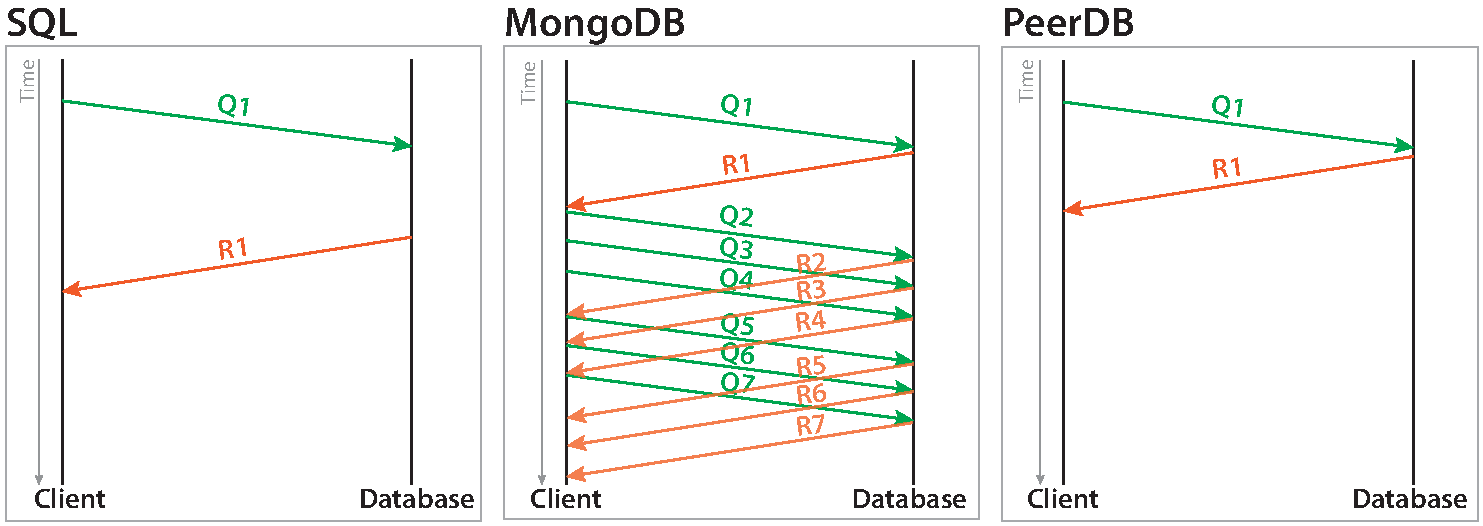
\includegraphics[width=0.9\columnwidth]{messages-many}
\caption{In traditional SQL, one query is needed to obtain data spawning multiple relations, but such results can be potentially large and time to compute joins is needed.
In MongoDB one has to create many subsequent queries to resolve relations, especially in many-to-many relations.
In PeerDB one has to simply fetch one document, with all relations already resolved, without any computation or communication among instances needed.}
\label{messages-many}
\end{figure}


Modern web frameworks like Meteor and DerbyJS introduced to the web developers community another family of database queries: reactive queries.
Using those frameworks you can make a database query where you receive results like you would for a normal query, but afterwards the query stays open and any changes to the results data is pushed to you in a reactive manner.
This allows you (or a framework you use) to respond to this changes in data.
For example, update a rendered template in a browser.
Programming in this way becomes much more declarative.

The downside is complexity a programer is faced with when making queries with joins.
While frameworks provide a simple to use primitive for making reactive queries against one MongoDB collection and receiving updates to documents in that collection as they are made for the open query, programming how manually resolved relations should respond to those updates in data is far from straightforward.
Community is slowly building libraries which are aiming to address these issues, but current solutions are made for specific type of queries and all share a common issue based on previously mentioned downside of manually resolving queries: high latency and number of queries.
As query results data is changed, queries for related documents have to be rerun again and again, even if the results of those new queries might not be different to previous ones, or even if only a smaller query for just a subset of documents would satisfy.

Thus, combination of joins in NoSQL databases with reactive queries pose a challenge to programers.
Luckily, we can observe that in many cases we are mostly interested only in few fields of a related document, again and again.
Instead of recomputing joins every time we read, we could use MongoDB's sub-documents feature to embed those fields along with the reference.
Instead of just storing the \verb|_id| of a related document, we could store also those few often used fields.
For example, if you are displaying blog posts, you want to display the author's name together with the blog post.
You will not really need only the blog post without the author name.
If an example blog post document looks like:

\begin{verbatim}
{
  "_id": "frqejWeGWjDTPMj7P",
  "body": "A simple blog post",
  "author": "yeK7R5Lws6MSeRQad",
  "tags": [
      "k7cgWtxQpPQ3gLgxa",
      "KMYNwr7TsZvEboXCw"
  ]
}
\end{verbatim}

Then the blog post with embedded common fields would look like:

\begin{verbatim}
{
  "_id": "frqejWeGWjDTPMj7P",
  "body": "A simple blog post",
  "author": {
    "_id": "yeK7R5Lws6MSeRQad",
    "name": "Wesley Crusher",
    "picture": "/img/yeK7R5Lws6MSeRQad.jpg"
  },
  "tags": [
    {
      "_id": "k7cgWtxQpPQ3gLgxa",
      "name": "announcement",
      "description": "Public announcements."
    },
    {
      "_id": "KMYNwr7TsZvEboXCw"
      "name": "test",
      "description": "Tests of the system."
    }
  ],
  "comments": [
    {
      "_id": "tMgj8mF2zF3gjCftS",
      "body": "A test comment."
    }
  ]
}
\end{verbatim}

Now we have to fetch only this one document and we have everything needed to display a blog post.
It is easy for us to query it and use it as any other document, with direct access to all subfields over which we can query as well.
For example, it is easy to query for all blog posts tagged with a given tag, provided that we have only its textual name to begin with.
We can make a MongoDB query \verb|{"tags.name": "test"}| to query all the documents tagged with tag \verb|test|.
The query can be reactive and we can easily get updates to it as data changes, without having to redo any queries for related documents.

Observe that blog post contains also comments data.
Each comment has a reference to a blog post of which a comment it is.
Information about a relation is thus stored in comment documents and not in posts themselves.
But we can embed this relation in the reverse direction as a list of subdocuments representing each comment referencing the blog post.

From the latency perspective such embedding of related documents makes queries much faster when reading.
Reactive queries do not have to requery related documents.
From the programmer's perspective this is much simpler to use because they can use familiar MongoDB queries directly.

Now, storing the author's name along with every blog post document brings an issue common when one is dealing with denormalized data.
What if user changes their name?
Then we have to update all those fields in documents referencing the user.
So we would have to make sure that anywhere in our code where we are changing the name, you are also updating fields in references.
What about changes to the database coming from outside of our code?

To address this issue and make easier for a programmer to embed subdocuments of related documents we designed and developer a layer on top of MongoDB called PeerDB.
Programmer can now in a declarative way specify relations between documents and which fields they would like to embed.
They have to define those references once and then PeerDB makes sure data stays in sync as it is changed across documents.
It does not matter where the changes come from, it will detect them and update fields in referenced sub-documents accordingly.

Instead of having to make recursive queries every time you read documents with related documents, PeerDB make those recursive queries once and store them into embedded documents.
The downside is that every modification to the data in the database triggers updates in documents in other collections.
While modifications to the document are stored quickly, changes have to propagate across all other documents.
To better understand performance characteristics of PeerDB we first present its implementation and then performance analysis approach and results.
Based on insights from performance analysis we follow by presenting an automatic algorithm to determine when to use embedding and when not to.
We conclude with our observations and discuss possible future work.
